\documentclass[11pt,makeidx,fleqn]{article}
\usepackage[intlimits,fleqn]{amsmath}
\usepackage{amssymb}
\usepackage{latexsym}
\usepackage{german}
\usepackage{graphics}
\usepackage{wrapfig}                            
                                            

\ifx\pdfoutput\undefined
  \usepackage[xdvi]{epsfig}
\else
  \usepackage{graphicx}
\fi

%\documentstyle[amstex,style,11pt]{article}
\setlength{\parindent}{0mm}
\setlength{\textwidth}{140mm}
\setlength{\textheight}{232mm}
\setlength{\topmargin}{-20mm}
\setlength{\headheight}{0in}
\setlength{\headsep}{1in}
%\setlength{\footheight}{0in}
\setlength{\footskip}{10mm}
\setlength{\oddsidemargin}{0.2in}
\setlength{\evensidemargin}{0.2in}
\setlength{\parskip}{4pt}                                
                               


\setcounter{secnumdepth}{5}   % bewirkt Aenderung der maximalen
                              % Kapitel-Nummerierung,
                              % hier von 3 (default) auf 5
\setcounter{tocdepth}{5}      % bewirkt Uebernahme der zusaetzlichen
                              % Kapitel-Ueberschriften ins Inhaltsverzeichnis
                                                                                  
            
%\usepackage{amsmath,amsthm,epsfig,amstext,amssymb,a4,makeidx,amscd,german}%amsfonts}
%\usepackage{graphicx,subfigure} %nickis Zeichnung??
%

\sloppy % fuer eine lockere Silbentrennung!!

\parindent0cm %keine Einrueckung nach Absatz
                
\pagestyle{myheadings} %kapitelueberschrift in Kopfzeile
\bibliographystyle{amsalpha}
%\DeclareGraphicsRule{.gif}{bmp}{}{}

%\styletitle{Interfacedesign}

\begin{document}

%***************************************************************************************

\newenvironment{list_sabina}{\begin{list}{$\bullet$}{\setlength{\labelwidth}{3mm} \setlength{\labelsep}{2mm} \setlength{\parsep}{1mm} \setlength{\topsep}{0mm} \setlength{\itemsep}{0mm}}}{\end{list}}
 
\newenvironment{sub_list_sabina}{\begin{list}{$\circ$}{\setlength{\labelwidth}{2.5mm} \setlength{\labelsep}{1mm} \setlength{\parsep}{1mm} \setlength{\topsep}{0mm} \setlength{\itemsep}{-1mm}}}{\end{list}}             

%***************************************************************************************


\pagestyle{empty}

\phantom{a}
\vspace{30mm}

\begin{center}
\underline{\underline{\Huge\bf Teil-Spezifikation}}\\[15mm]
{\Large\bf Multimediale}\\[2ex]
{\Large\bf Mathematikausbildung}\\[2ex]
{\Large\bf f"ur Ingenieure}\\[14ex]
{\Large\bf Interfacedesign}
\item \end{center}

\vspace{22mm}

\begin{center}
{\large \textbf{Autoren:}}\\[2.5ex] 
{\large Sabina Jeschke -- Erhard Zorn}
\end{center}


\vspace{10mm}

\begin{center}
{\large\bf Stand: Berlin, \today}
\end{center}

\vspace{5mm}

\begin{tabular}{ll}
\textsf{Datum:}&\verb+$Date: 2004/01/28 19:12:08 $+\\ % Wird vom cvs eingetragen
\textsf{CVS-Version:}&\verb+$Revision: 1.4 $+\\ % Wird vom cvs eingetragen
\textsf{CVS-Source:}&\verb+$Source: /net/mumie/cvs/styles/interfacedesign/titel.tex,v $+\\ % Wird vom cvs eingetragen
\end{tabular}

\newpage

\phantom{was auch immer...}

\setcounter{page}{0}

\clearpage

\pagestyle{plain}

%**************************************************************************




\clearpage

\tableofcontents
\clearpage


\section{Name und Begleitfiguren}\label{}

Das Projekt hei"st ``Mumie''\footnote{Aktuell bem"uhen wir uns, die
domain zu erwerben...}.

Es gibt \textbf{zwei} Begleitfiguren:

\begin{list_sabina}
\item
\textbf{Mumie}:\\
Die Mumie ist der ``Hauptcharakter''.
Sie unterst"utzt den User  mit Schwerpunkt auf den \textit{fachlichen} Hinweisen.
\item
\textbf{Skarab"aus}:\\
Der Skarab"aus ist Partner der Mumie (etwa bei Dialogen), er
unterst"utzt au"serdem den User mit Schwerpunkt auf den 
\textit{organisatorischen} Anweisungen.
\end{list_sabina}


\begin{figure}[h]
\begin{center}
\ifx\pdfoutput\undefined
  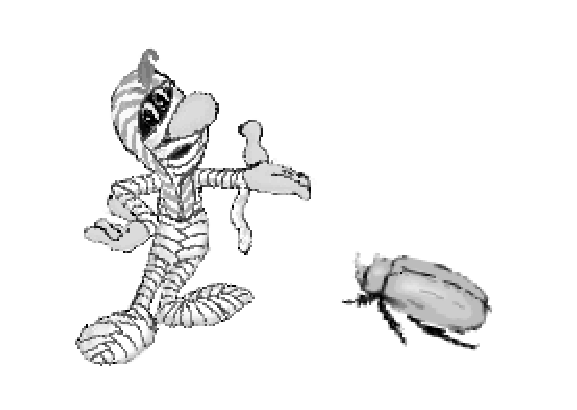
\epsfig{file=Skizzen/my_combi_02.eps, height = 5cm}
\else
  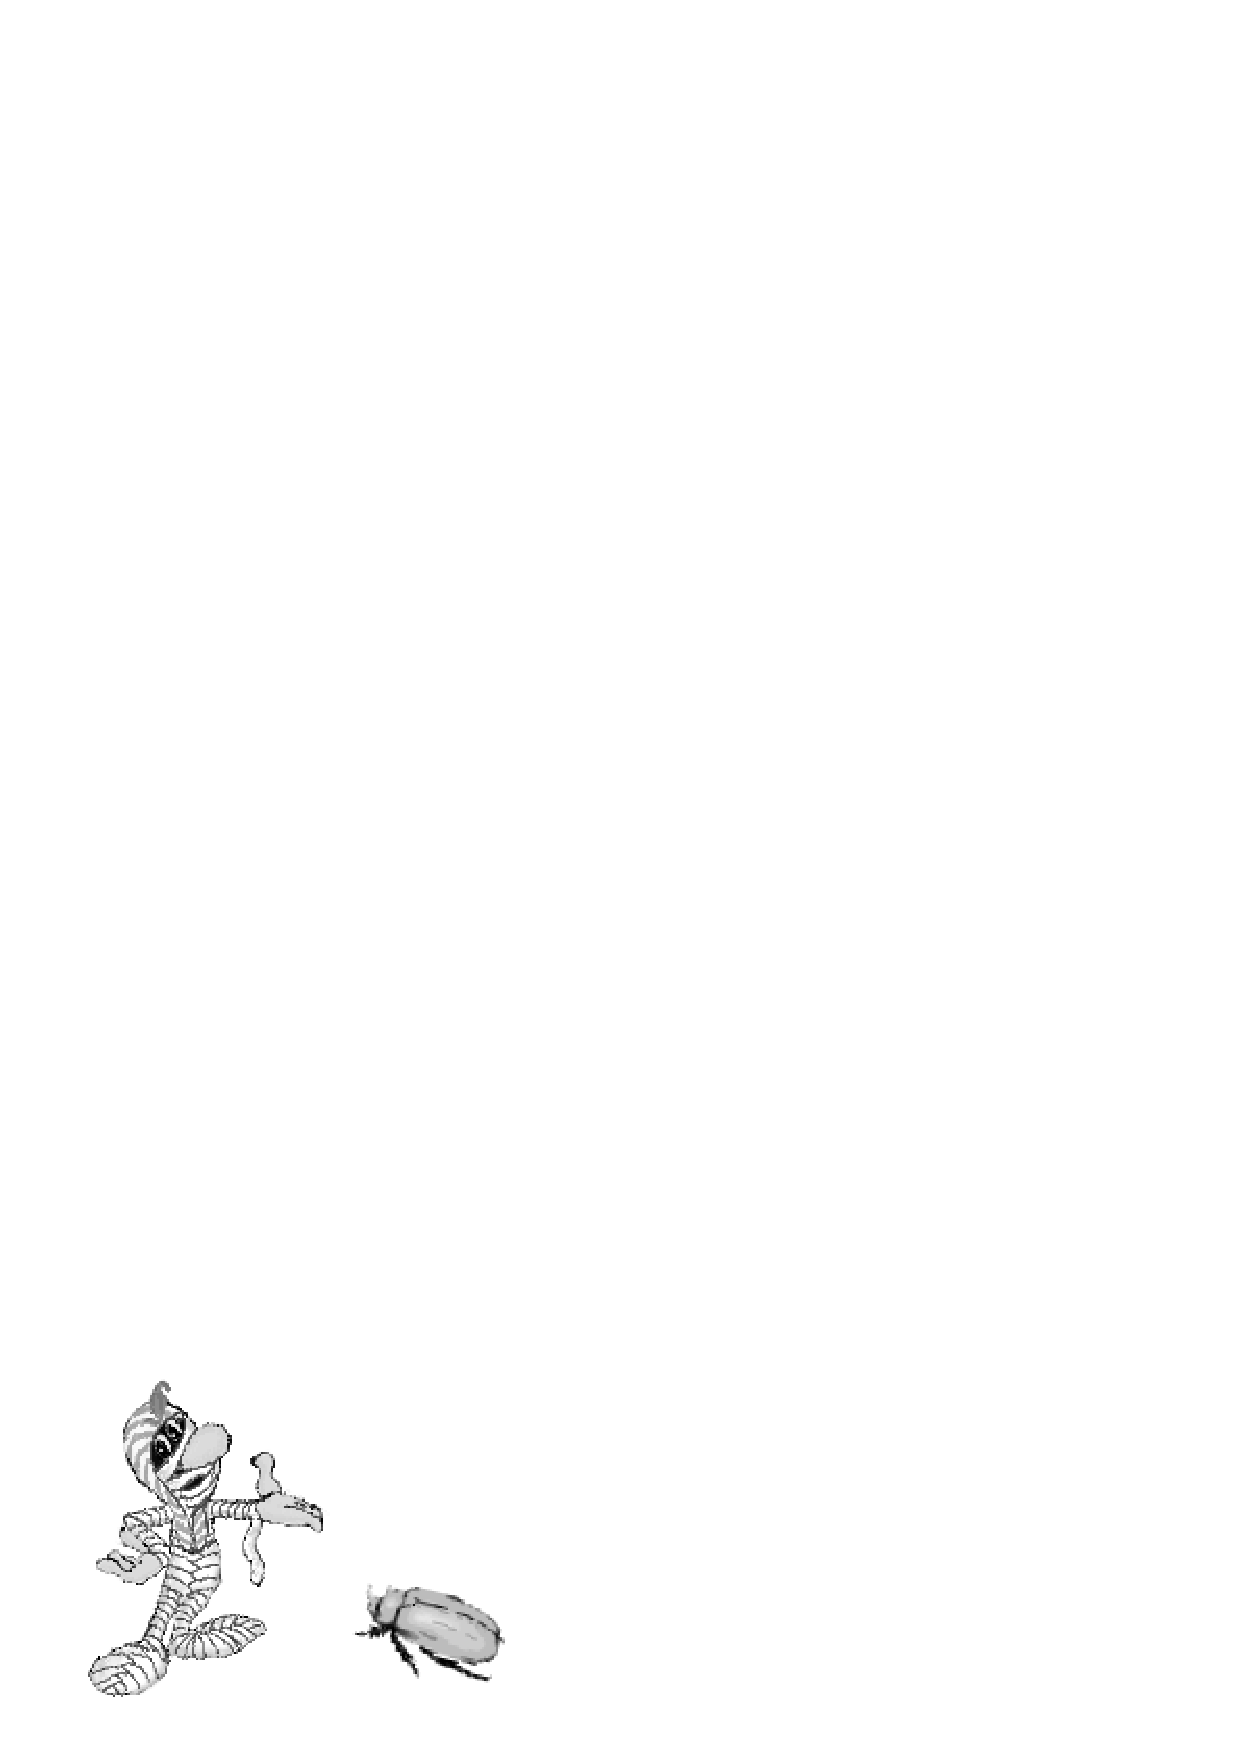
\includegraphics{Skizzen/my_combi_02.pdf}
\fi
\caption{Die Begleitfiguren (nur ``funktionale Skizze'')}
\end{center}
\end{figure}


Die Eins"atze der Begleitfiguren sind toolspezifisch und werden 
daher jeweils in den entsprechenden Tools beschrieben.


\vspace{10mm}

{\footnotesize\textit{Ideen/Layoutvorschl"age: Die Figuren sollten
comicartige Figuren sein und in verschiedenen Ausf"uhrungen (sitzend,
stehend, mit Buch in der Hand, auf fliegendem Teppich, ...), mit
verschiedener Gestik/Mimik (lachend, irristiert, sich die Haare
raufend, ...) und animiert verwenden werden k"onnen. Die Mumie
k"onnte etwa Miraculix oder auch Gandalf nachempfungen sein... weise,
aber auch viel Charakter. Eingewickelt nat"urlich. Der Skarab"aus
k"onnte sich an Kassiopeia (Michael Ende, Momos Schildkr"ote)
anlehnen: die hatte bisweilen eine Leuchtschrift auf dem R"ucken...}}


\clearpage


\section{Entr\'{e}e}\label{entree}

%********************************************************************************

\subsection{Portalseite}

Stichworte f"ur die Portalseite der Mumie sind: 

\begin{list_sabina}
\item
\textbf{Design/Graphik:} ansprechend, sch"on, professionell\\
"Ubersicht "uber Haupttools, wenige Buttons
\item
\textbf{Stimmung:} Universalit"at der Mathematik, multikulturell
\item
\textbf{Performance:} kurze Ladezeiten, Lauff"ahigkeit unter bel.
Browsers mu"s mindestens f"ur die Portalseite (und die direkt auf sie
folgenden, eher organisatorisch orientierten Seiten) absolut
sichergestellt sein
\item
\textbf{Inhalt:} Projektname ``Mumie'', Integration der tragenden 
Charaktere (Begleiter), Haupttools, Links (s. unter ``Funktionalit"at'')
\item
\textbf{Funktionalit"at:} Zugang zu
        \begin{sub_list_sabina}
        \item
        Vollversion (mit Authentifizierung) und Demoversion
        \item
        Helppages
        \item
        Infopages
        \item
        Direktzugang zu Haupttools (nachgeschaltete Authentifizierung)
        \end{sub_list_sabina}
\end{list_sabina}

\begin{figure}[h]
\begin{center}
\ifx\pdfoutput\undefined
  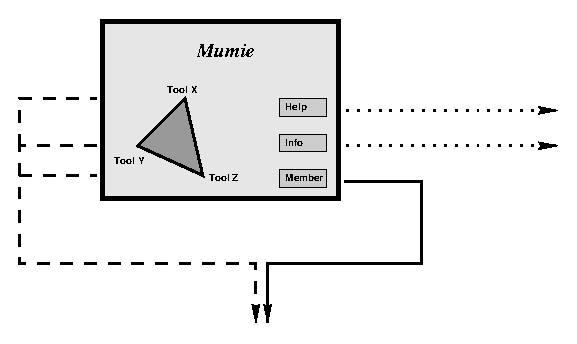
\epsfig{file=Skizzen/portal_main.eps}
\else
  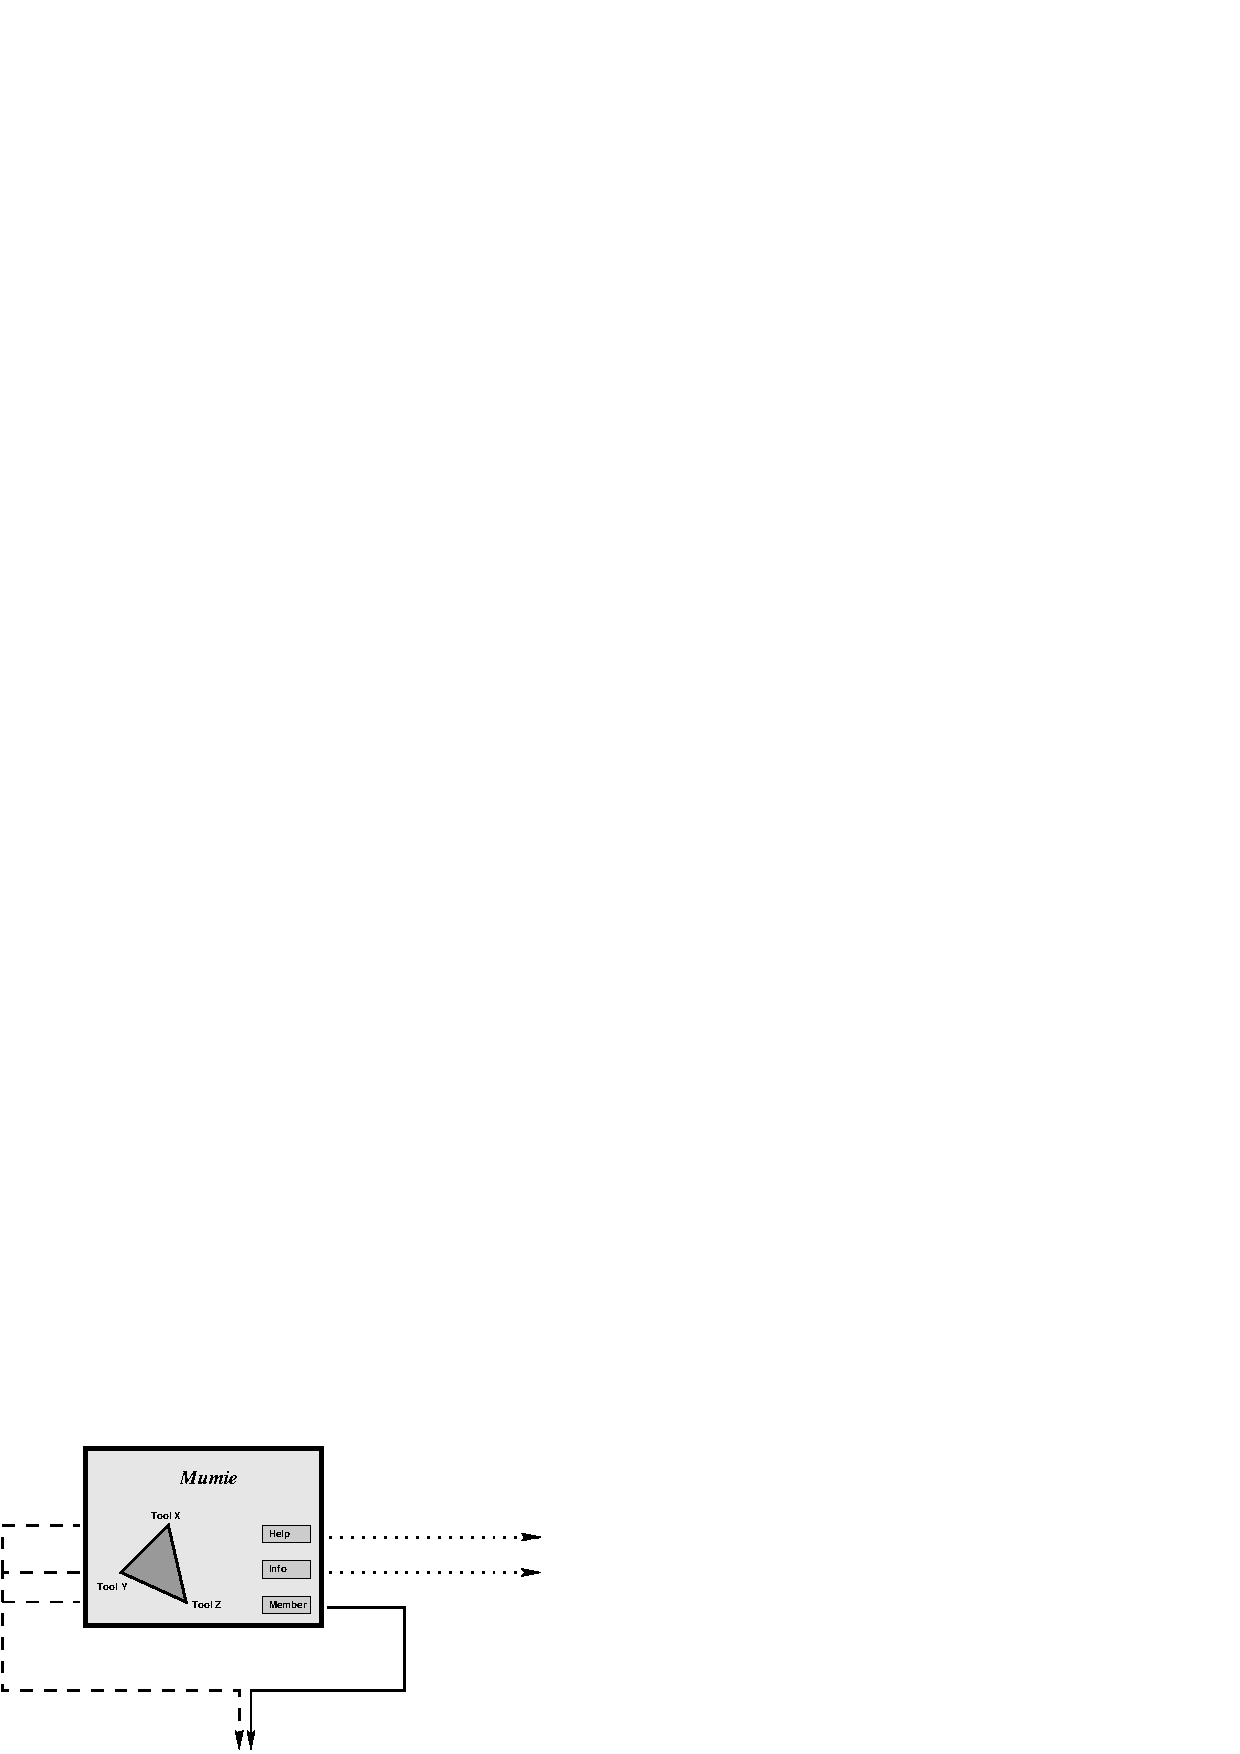
\includegraphics{Skizzen/portal_main.pdf}
\fi
\caption{"Ubersicht "uber das Portal und die direkten Folgeseiten}
\end{center}
\end{figure}
 
Die Logos der beteiligten ProjektPartner-Universit"aten k"onnen,
m"ussen aber nicht unbedingt Bestandteil der Einstiegsseite sein,
zumal etliche andere Verbundprojekte auch davon Abstand nehmen und
sich diese Informationen au"serdem unter direkt von der Portalseite
aus zu erreichenden den Infopages (Kap. \ref{kap:info_pages}) sogar
wesentlich detaillierter pr"asentieren. Hier sollte zun"achst
R"ucksicht auf die graphische Gesamtgestaltung genommen werden.

%********************************************************************************

\clearpage

%********************************************************************************

\subsection{Zug"ange}

Es werden grunds"atzlich zwei Zugangsformen vorgesehen: die ``Vollversion''
(mit Authentifizierung) und eine sog. ``Demoversion''\footnote{Die Demoversion
  beinhaltet einige besonders ansprechende und gelungene Beispiele aus dem
  Projekt und verweist weiter auf die Authentifizierungsseite.  Der Demozugang
  wird vorl"aufig \textit{ohne Inhalte} als Dummy-Zugang realisiert.} (ohne
Identifikation oder
Authentifizierung).

Beide Zugangsformen werden von der Portalseite aus "uber zwei verschiedene
Wege erreicht:
\begin{list_sabina}
\item
\textbf{"uber den Memberbutton} 
\item
\textbf{"uber das Anklicken eines Tools} 
\end{list_sabina}


\subsubsection{Zugang "uber Memberbutton}

Der Usert wird zu einer dreigeteilten Authentifizierungsseite geleitet
(frames; da die einzelnen Teile noch in anderen Kontexten Anwendung finden
k"onnen):

\begin{list_sabina}
\item
\textbf{Authentifizierungsbereich:} (in Skizzen rechts oben)\\
Userid und password werden abgefragt, der Demozugang wird "uber userid
``demo'', password ``demo'' erreicht (dazu existiert ein
erl"auternder Text auf der Seite).
\item
\textbf{Anmeldebereich:} (in Skizzen rechts unten)\\
Liegt (noch) kein userid/password vor, so kann hier ein
solcher Zugang beantragt werden\footnote{Die Vergabe eines Zuganges
erfolgt \textit{nicht} automatisch, sondern durch einen
``Mumienadministrator''.}. Der Neu-User wird zu einer Formular-Seite
geleitet (notwendige Angaben t.b.s.); diese enth"alt die "ublichen
Fehlerabfragen und Best"atigungen beim Absenden.\\
Dieser Bereich beeinhaltet ebenfalls einen erl"auternden Text zu den
grunds"atzlichen Regelungen und Grundlagen f"ur die Vergabe von Zug"angen.
\item
\textbf{Orientierungsbereich:} (in Skizzen links)\\
Der Orientierungsbereich wird i.w. nur mit ansprechender Graphik gestaltet.\\
(Die eigentliche Bedeutung erh"alt dieser Bereich erst beim Zugang
"uber eines der Tools, siehe Kap. \ref{kap:toolzugang}.) 
\end{list_sabina}

\begin{figure}[h!]
\begin{center}
\ifx\pdfoutput\undefined
  \epsfig{file=Skizzen/authent_page_member.eps}
\else
  \includegraphics{Skizzen/authent_page_member.pdf}
\fi
\caption{Authentifizierung "uber den Memberbutton}
\end{center}
\end{figure}



Bei erfolgreichem login erh"alt der User eine Auswahl:

\begin{list_sabina}
\item
\textbf{zur einer zentralen Einstiegs-"Ubersichtsseite der Mumie}\\
(Default nach Demo-Zugang)
        \begin{sub_list_sabina}
        \item
        Zugang zu Haupttools
        \item
        Zugang zum Userprofil
        \end{sub_list_sabina}
\item
\textbf{zur Startseite}
        \begin{sub_list_sabina}
        \item
        des Lerntools
        \item
        des "Ubungstools
        \item
        ...
        \end{sub_list_sabina}
\item
\textbf{zur"uck zur letzten besuchten Seite} (user-spezifisch)
        \begin{sub_list_sabina}
        \item  
        global
        \item
        des Lerntools
        \item
        des "Ubungstools
        \item
        ...
        \end{sub_list_sabina}
\item
\textbf{zu meinem User-Profil}\\
(to be specified)
\end{list_sabina}

\begin{figure}[h!]
\begin{center}
\ifx\pdfoutput\undefined
  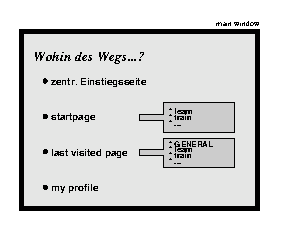
\epsfig{file=Skizzen/weg_auswahl.eps}
\else
  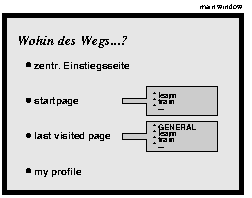
\includegraphics{Skizzen/weg_auswahl.pdf}
\fi
\caption{Auswahl nach erfolgreicher Authentifizierung bei Verwendung
des Memberbuttons}
\end{center}
\end{figure}


\clearpage

\subsubsection{Direktzugang "uber ein Tool}\label{kap:toolzugang}

Es werden nur die Unterschiede zum Zugang "uber den Memberbutton skizziert:

Der Usert wird zu wieder zu der dreigeteilten Authentifizierungsseite
geleitet; der Orientierungsbereich enth"alt nun ein ``Abstract'' aus Graphik
und Text zu dem Tool, das er gew"ahlt hat.

Bei erfolgreichem login erh"alt der User keine weitere Auswahl, sondern wird
direkt auf die letzte besuchte Seite des Tools geleitet, das er angew"ahlt
hat.  Damit erreicht er diesen Punkt nach nur \textit{einem} Zwischenschritt
(der Authentifizierung, die nicht eingespart werden kann).

\begin{figure}[h]
\begin{center}
\ifx\pdfoutput\undefined
  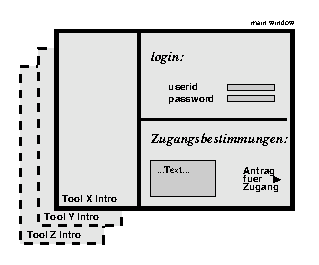
\epsfig{file=Skizzen/authent_page_tool.eps}
\else
  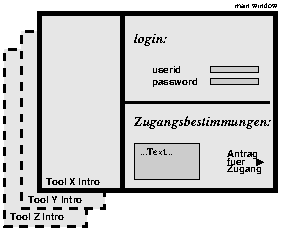
\includegraphics{Skizzen/authent_page_tool.pdf}
\fi
\caption{Authentifizierung "uber ein Tool}
\end{center}
\end{figure}


\subsubsection{Fehlermeldung bei der Authentifizierung}

Bei nicht-erfolgreichem login erh"alt der User eine entsprechende
Fehlermeldung sowie erneute Einlog-M"oglichkeit (die urspr"ungliche
Authentifizierungsseite erscheint wieder, erg"anzt um die
Fehlermeldung und Erl"auterungen, Link zur Kontaktaufnahme mit dem
Webmaster etc.).

\begin{figure}[h]
\begin{center}
\ifx\pdfoutput\undefined
  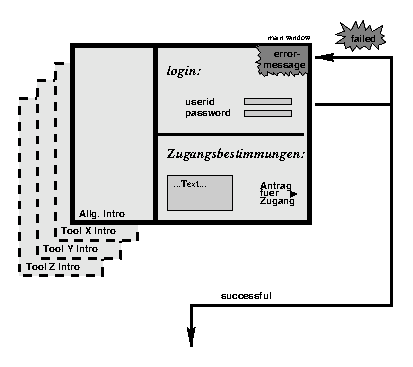
\epsfig{file=Skizzen/authent_page_error.eps}
\else
  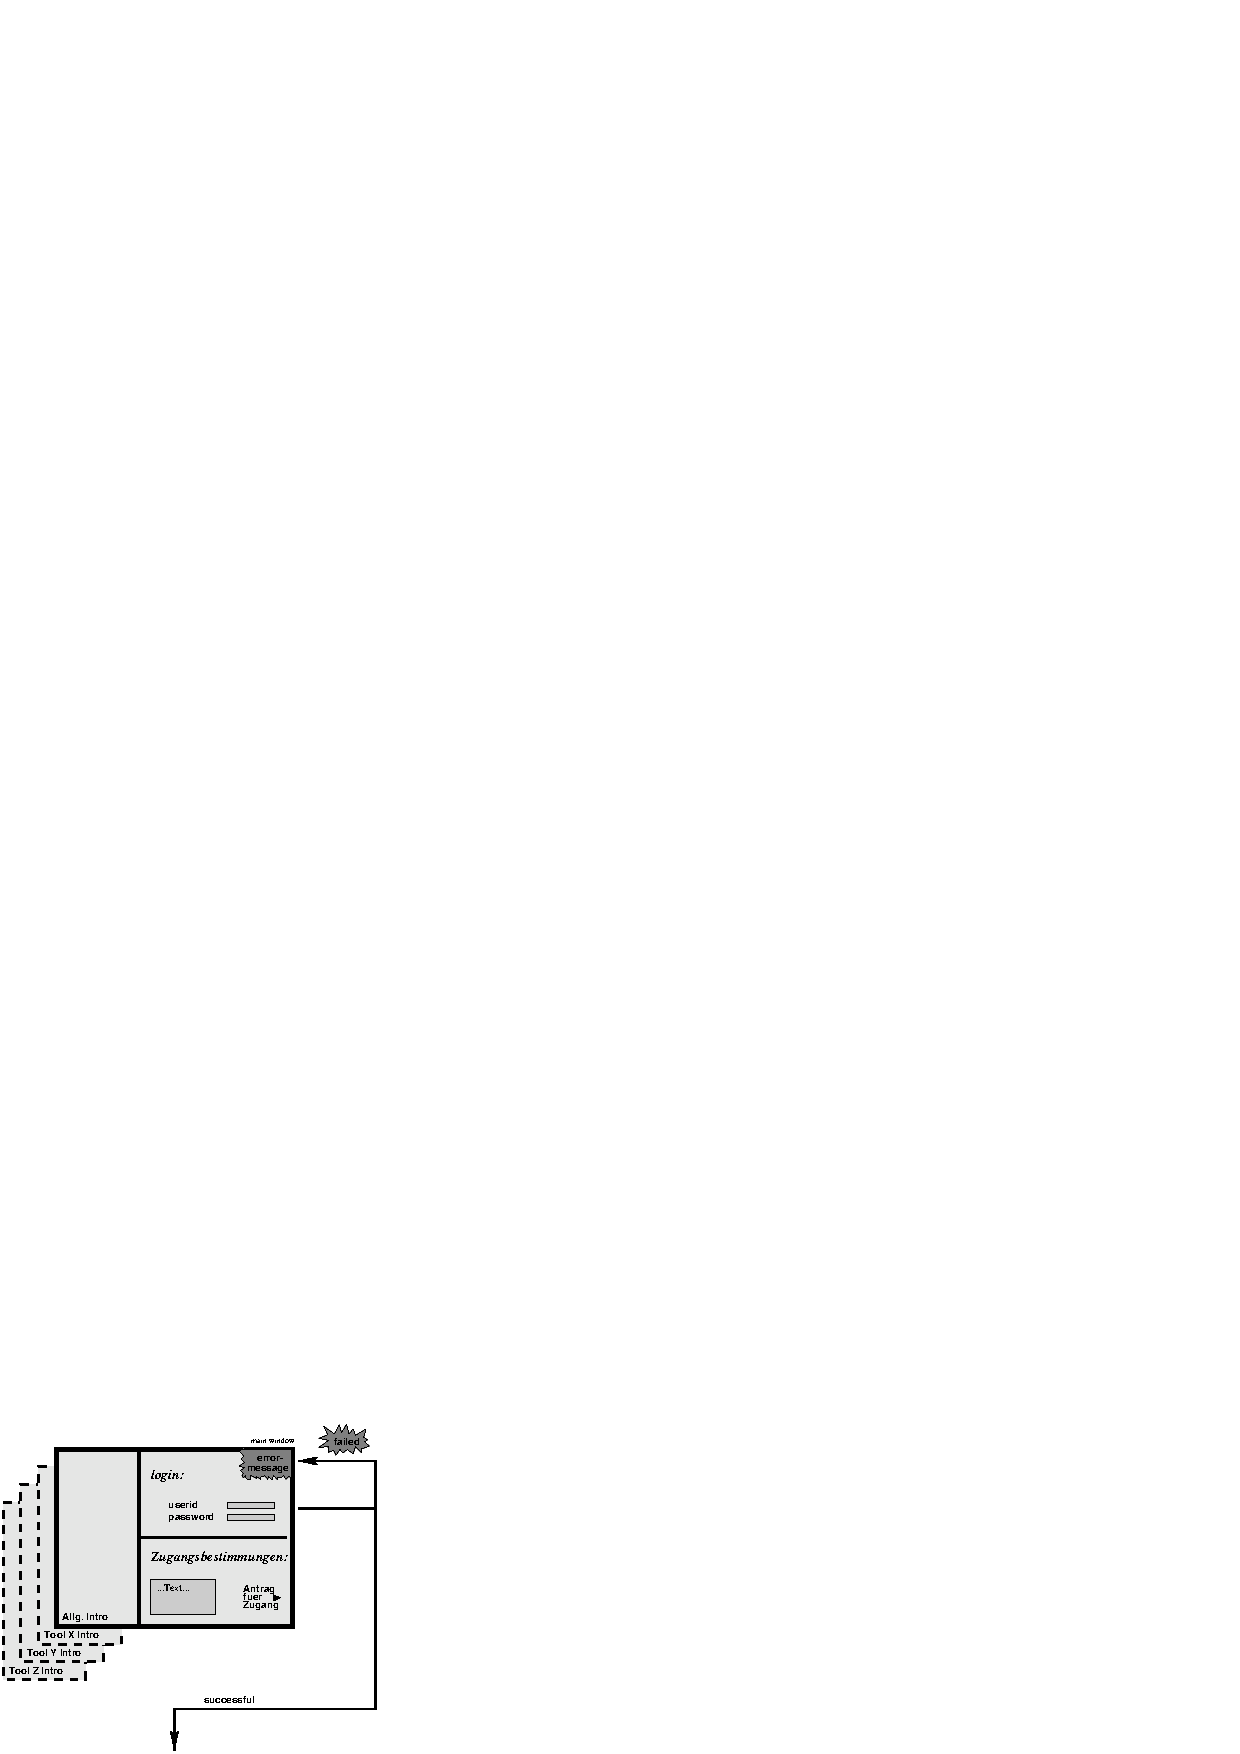
\includegraphics{Skizzen/authent_page_error.pdf}
\fi
\caption{Fehlermeldung bei Authentifizierung "uber Memberbutton \textit{und} Tool}
\end{center}
\end{figure}

\clearpage

\subsubsection{Graphische "Ubersicht "uber die Zug"ange}

\begin{figure}[h!]
\begin{center}
\ifx\pdfoutput\undefined
  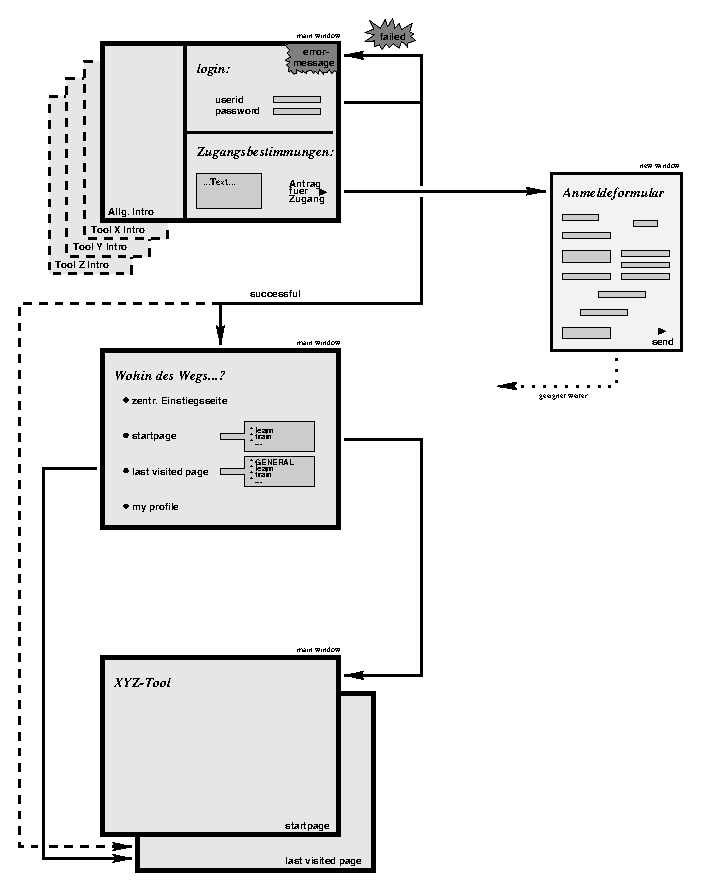
\epsfig{file=Skizzen/authent_page_overview.eps}
\else
  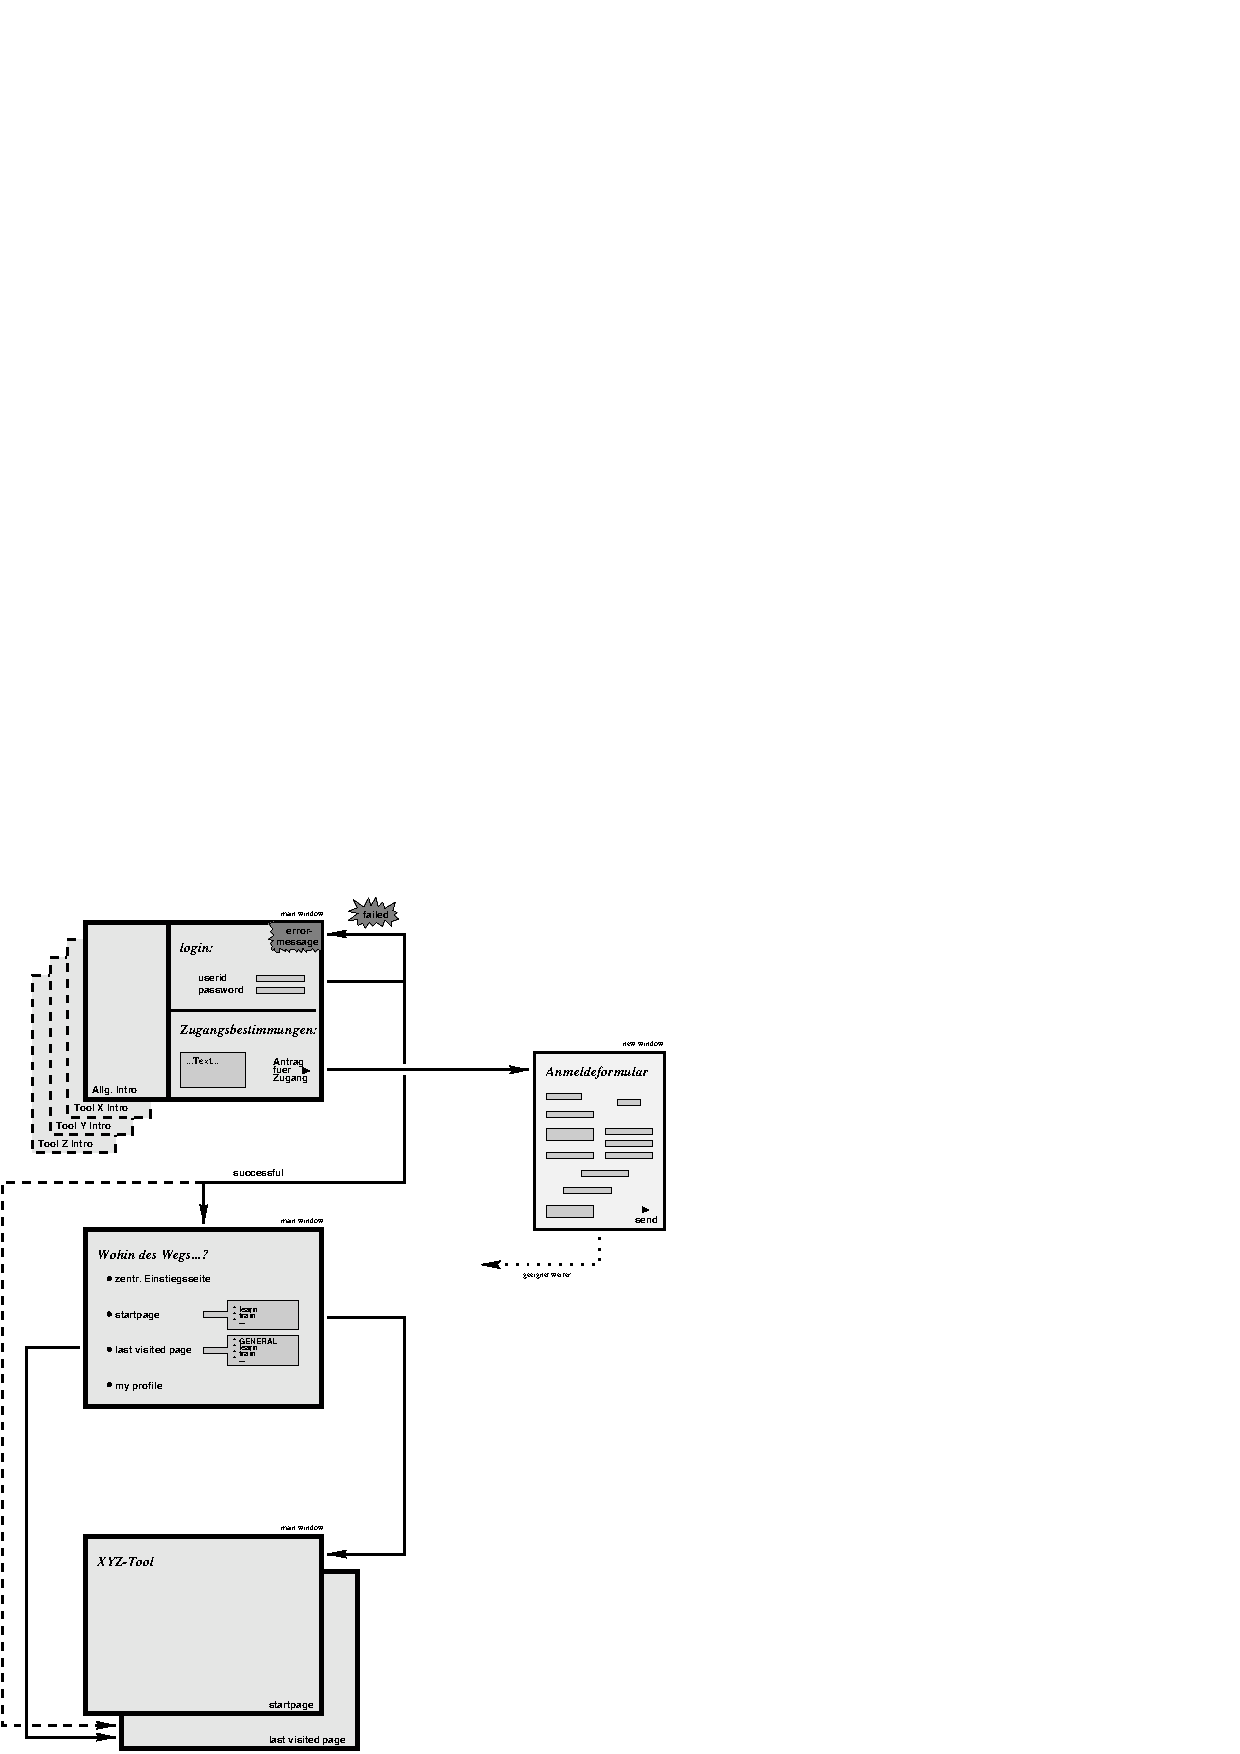
\includegraphics{Skizzen/authent_page_overview.pdf}
\fi
\caption{Authentifizierung "uber Memberbutton \textit{und} Tool}
\end{center}
\end{figure}
 
%********************************************************************************

\clearpage

%********************************************************************************

\subsection{Help-Pages}

Die Help-Pages werden an die graphisch-thematische Idee der Einstiegsseite 
angelehnt.\\
Sie zerfallen in folgende Bereiche:

\begin{list_sabina}
\item
\textbf{"Ubersichtsseiten:}
Die oberste Hierarchie der Help-Pages gibt eine "Ubersicht in die
gesamte Lernsoftware ``Mumie'', insbesondere "uber
die bestehenden Tools und deren Zusammenh"ange.
\item
\textbf{Toolspezifische Seiten:}
Die zentralen Teile der Help-Pages sind toolspezifisch und werden daher erst
mit fortschreitender Entwicklung der Tool differenziert beschrieben.
\item
\textbf{Seiten f"ur externe Helferlein:}
Der Einstieg eventuell angeschlossener/integrierter Tools (wie MathLab,
Mathematica, ...) und anderer potentiell sinnvoller Erg"anzungen
(Programmiersprachen, ...) wird durch (kurze) Dokumentationen unterst"utzt.
\end{list_sabina}

Bei den Help-Pages mu"s sorgf"altig zwischen ``organisatorischen'' und
``fachlichen'' Anwendungen unterschieden werden.

\vspace{10mm}

t.b.s. in detail

%********************************************************************************

\clearpage

%********************************************************************************

\subsection{Info-Pages}\label{kap:info_pages}

Die Info-Pages zerfallen in folgende Bereiche:

\begin{list_sabina}
\item
\textbf{Allgemeine Informationen:}
F"orderung, wer, wann, was, aktueller Stand, geplante Ausbaustufen, ...
\item
\textbf{Links zu beteiligten Partnern:}
Links zu den Universit"aten, zu den lokalen Projektleiterern, 
zu den Mitarbeitern, ...
\item
\textbf{Hintergrundinfos:}
Artikel etc.
\end{list_sabina}

\vspace{10mm}

t.b.s. in detail

%********************************************************************************

\clearpage

%********************************************************************************

\subsection{Graphische "Ubersicht Entr\'{e}e-Bereich}

%Die skizzierten Zugangswege sind die ``kanonischen''.\\
%Zus"atzlich werden, um der Nichtlinearit"at des Mediums
%und den verschiedenen Userbed"urfnissen gerecht zu werden,
%``quer verlaufende'' zus"atzlich (i.w. aber ohne gro"sen
%Zusatzaufwand) realisiert:

\begin{figure}[h!]
\begin{center}
\ifx\pdfoutput\undefined
  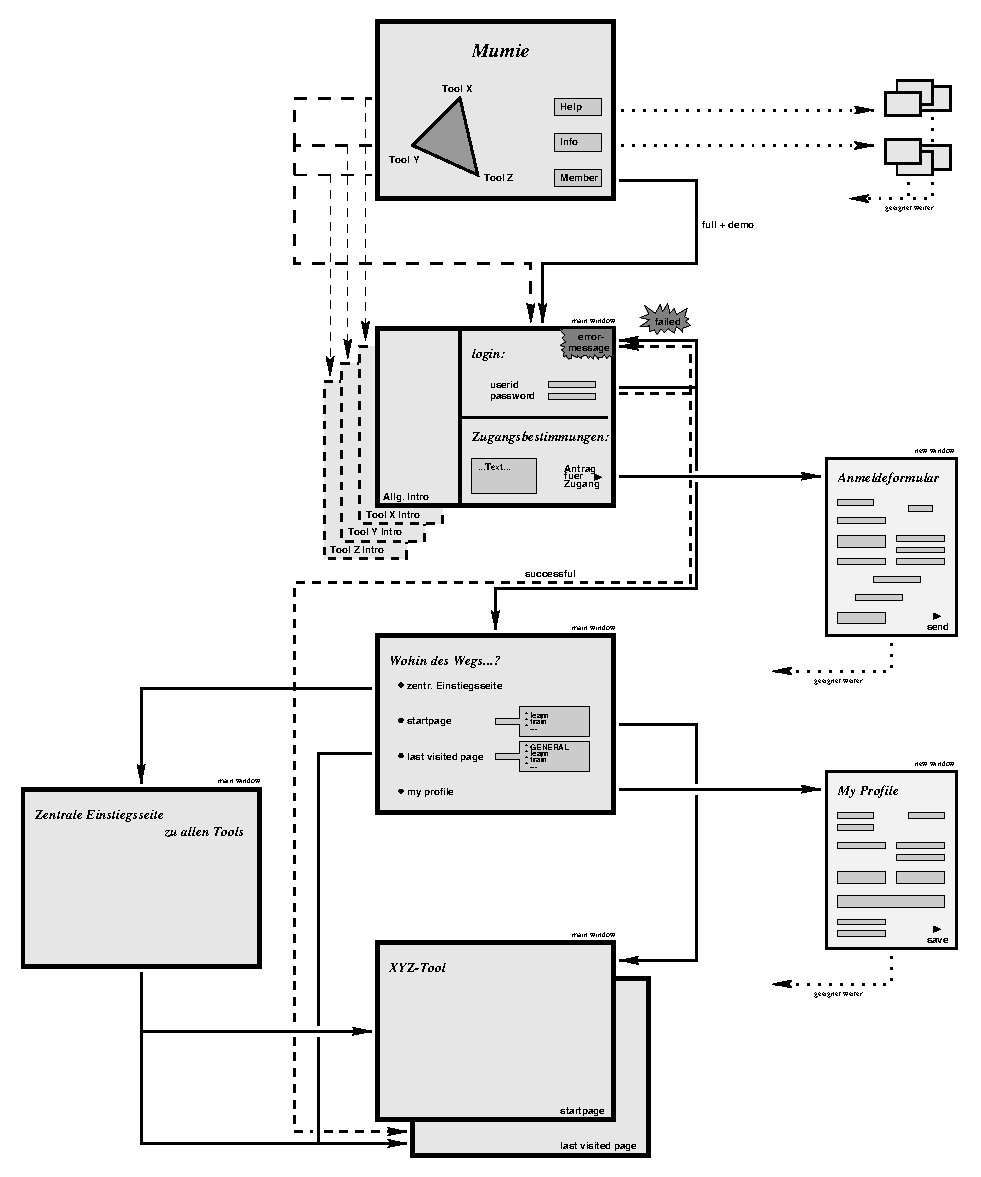
\epsfig{file=Skizzen/overview_portal.eps}
\else
  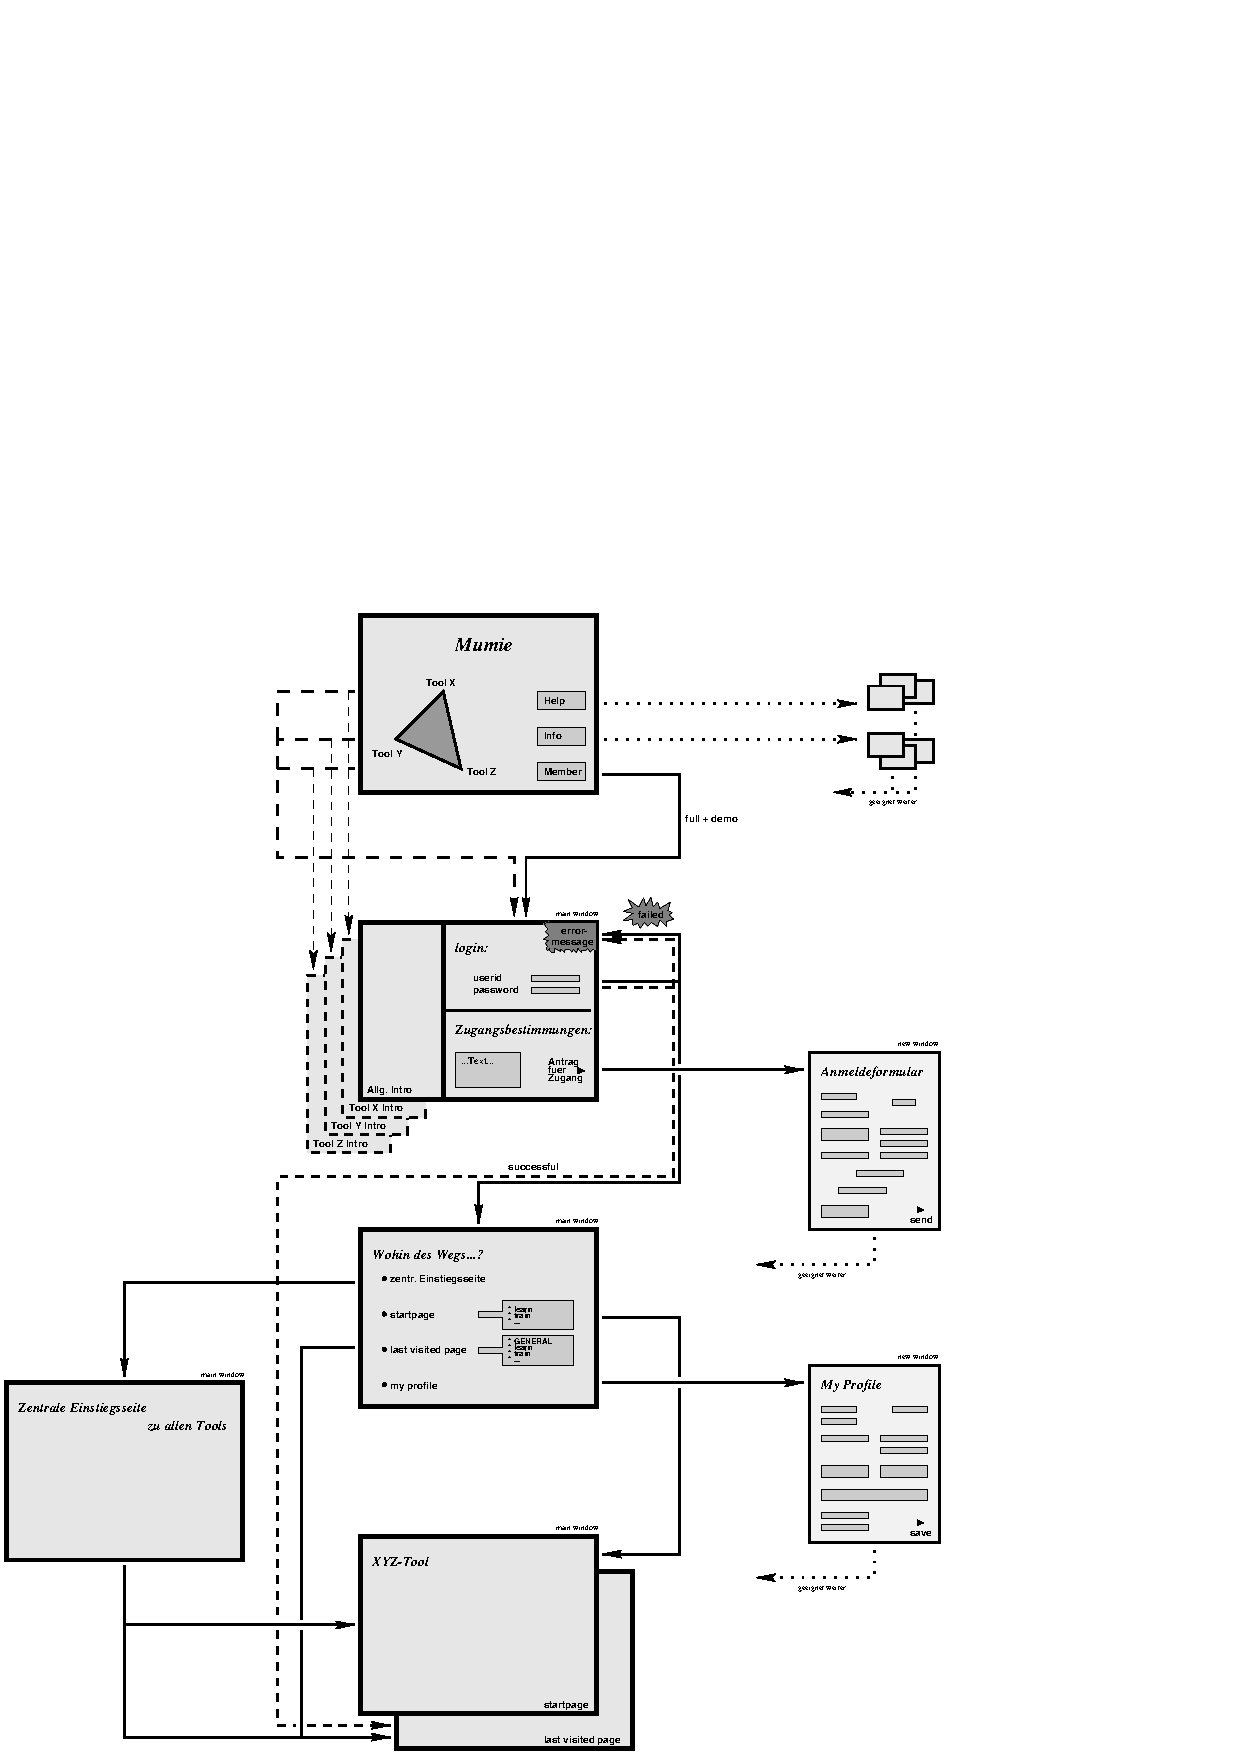
\includegraphics{Skizzen/overview_portal.pdf}
\fi
\caption{"Ubersicht "uber das Portal und die  Folgeseiten 1. und 2, Stufe}
\end{center}
\end{figure}
 















\clearpage


\section{Lerntool}\label{lerntool}

%********************************************************************************

\subsection{Overview}\label{overview}
 
 
Im Lernteil des Mumie-Projektes unterteilt sich das
\textbf{Haupt}browserfenster in folgende Bereiche:
 
\begin{list_sabina}
        \item \textbf{zentrale Men"uleiste} (f"ur globale Optionen)
        \item \textbf{Navigationsbereich} (f"ur die interaktive Pr"asentation des speziellen Moduls)
        \item \textbf{zentrale Inhaltsfenster} (f"ur den inhaltlichen ``Hauptinput'')
\end{list_sabina}                                                                                     

\begin{figure}[h]
\begin{center}
\ifx\pdfoutput\undefined
  \epsfig{file=Skizzen/gesamtszenario_01.eps, height = 5cm}
\else
  \includegraphics{Skizzen/gesamtszenario_01.pdf}
\fi
\caption{Layout der Hauptansicht im Lerntool}
\end{center}
\end{figure}                                   

Im folgenden werden diese Bereiche im Detail beschrieben.
                                  
%********************************************************************************

\clearpage

%********************************************************************************

\subsection{Zentrale Men"uleiste}

Die zentrale Men"uleiste besteht strukturell aus zwei Teilen:

\begin{list_sabina}
        \item \textbf{Graphischer Teil} f"ur Wechsel zwischen den
          verschiedenen Tools
        \item \textbf{Men"uteil} f"ur alle "ubrigen Funktionalit"aten\\
          (die i.a. weitere Unterstrukturen haben)
\end{list_sabina}                                                                                     

Die zentrale Men"uleiste ist (wie der Name sagt) ``zentral'' f"ur alle Tools der Mumie, \\
die Unterstrukturen des integrierten Pull-Down k"onnen jedoch verschieden
sein.\\
F"ur das Lerntool ergibt sich folgendes Bild:

\begin{figure}[h]
\begin{center}
\ifx\pdfoutput\undefined
  \epsfig{file=Skizzen/zent_menue.eps}
\else
  \includegraphics{Skizzen/zent_menue.pdf}
\fi
\caption{Layout der zentralen Men"uleiste}
\end{center}
\end{figure}                                   

Als ``Vorbild'' f"ur die Raumaufteilung zwischen Graphik- und Men"uteil und
auch f"ur die ungef"ahre Gr"o"se kann \verb?www.heute.t-online.de? gelten.
Der Graphische Teil sollte die Layout-Idee der Einstiegsseite aufgreifen.\\
Die detaillierte Entwicklung der Zentralen Men"uleiste ist damit der
Entwicklung des Gesamtlayouts zeitlich nachgeordnet (eventuell vereinfachte 
Dummyversion erstellen?).

%********************************************************************************

%\clearpage

%********************************************************************************

\subsection{Navigationsframe}

Details zum Navigationsframe werden derzeit in der separaten Spezifikation
``Navigationsframe'' (S.~Jeschke/E.~Zorn, November 2001) beschrieben.\\
Hier daher nur eine Zusammenfassung:

Der Navigationsbereich wird auf zwei verschiedene Weisen realisiert:

\begin{list_sabina}
        \item \textbf{Navigationsnetz}: Die Netzdarstellung erlaubt das orientierte
          Navigieren im gew"ahlten Kurs, stellt aber zus"atzlich weitere
          Elemente und alternative Wege dar, die jederzeit mit angew"ahlt
          werden k"onnen. \\
          Die Netzstruktur dient insbesondere der Vermittlung von
          mathematischen Zusammenh"angen: die logischen Abh"angigkeiten der
          Elemente werden durch eine Strichart (``logisches Netz''), 
          der gew"ahlte Kurs durch eine zweite Strichart (``Kurspfad'')
          dargestellt. Forward/Backward-Aktionen beziehen sich stets
          auf den Kurspfad.
        \item \textbf{lineare Navigation:} Die lineare Darstellung (Modell
          etwa wie ein U-Bahn-Plan f"ur eine einzige Linie) stellt nur die
          Elemente des Modules dar, die f"ur den gew"ahlten Kurs vorgesehen
          sind. Alternative Wege und/oder weitere vorhandene Elemente sind in
          dieser Darstellung unsichtbar.\\
          Die lineare Navigation dient insbesondere dem Ziel, dem 
          ``Lost-in-Cyberspace''-Effekt entgegenzuwirken.
\end{list_sabina}


Ausgangspunkt f"ur die Darstellung ist zun"achst das Navigationsnetz (hier
wird auf Alternativen erst aufmerksam gemacht, deren Existenz andernfalls
nicht sichtbar ist). Zwischen den beiden Navigationsformen kann zu jeden
Zeitpunkt geswitched werden (Karteikartensytem am oberen Rand des
Navigationsbereiches).
Zwischen den verschiedenen Ansichten (Navigationsnetz und Lineare
Navigation) wird durch ein Karteikartensystem hin- und hergeschaltet,
welches dar"uber hinaus weitere Karten verwaltet:

\begin{list_sabina}
        \item \textbf{1. Navigationsnetz}
        \item \textbf{2. Lineare Navigation}
        \item \textbf{3. Summary:}
        Zusammenfassung eines Modules \\
        (Stichwort: Vorschl"age nach V. En"s, to be specified)
        \item \textbf{4. Notes:}
        eigene Bemerkungen und Statusanzeigen, angelegt vom User \\
        (Stichwort: nach Linguistikprojekt, gesehen in K"oln, to be specified)
\end{list_sabina}

Die Karten werden durch Icons gekennzeichnet.\\
Aktivieren einer Karteikarte markiert deren Auswahl durch farbliche
"Anderung, highlighting etc.

Layouttechnisch muss das Auftreten von mindestens zwei weiteren
Karteikarten eingeplant werden (insbesondere auch im Hinblick auf die
"ubrigen Tools).

\begin{figure}[h]
\begin{center}
\ifx\pdfoutput\undefined
   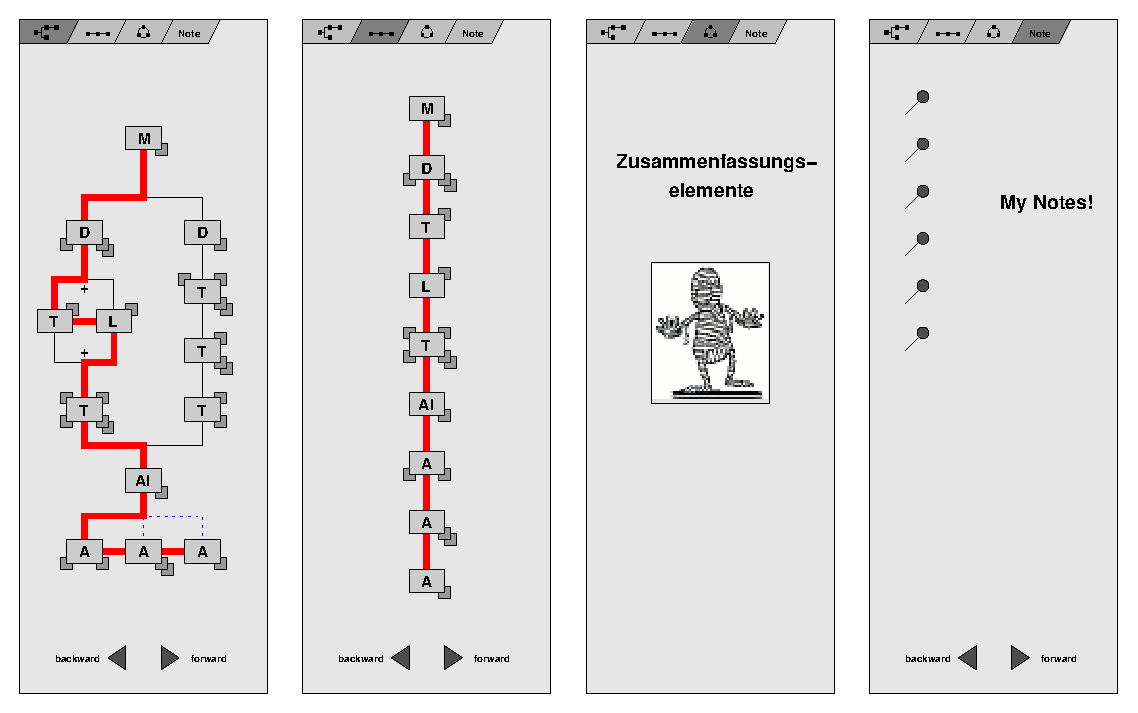
\epsfig{file=Skizzen/all_cards.eps, height=80mm} 
\else
  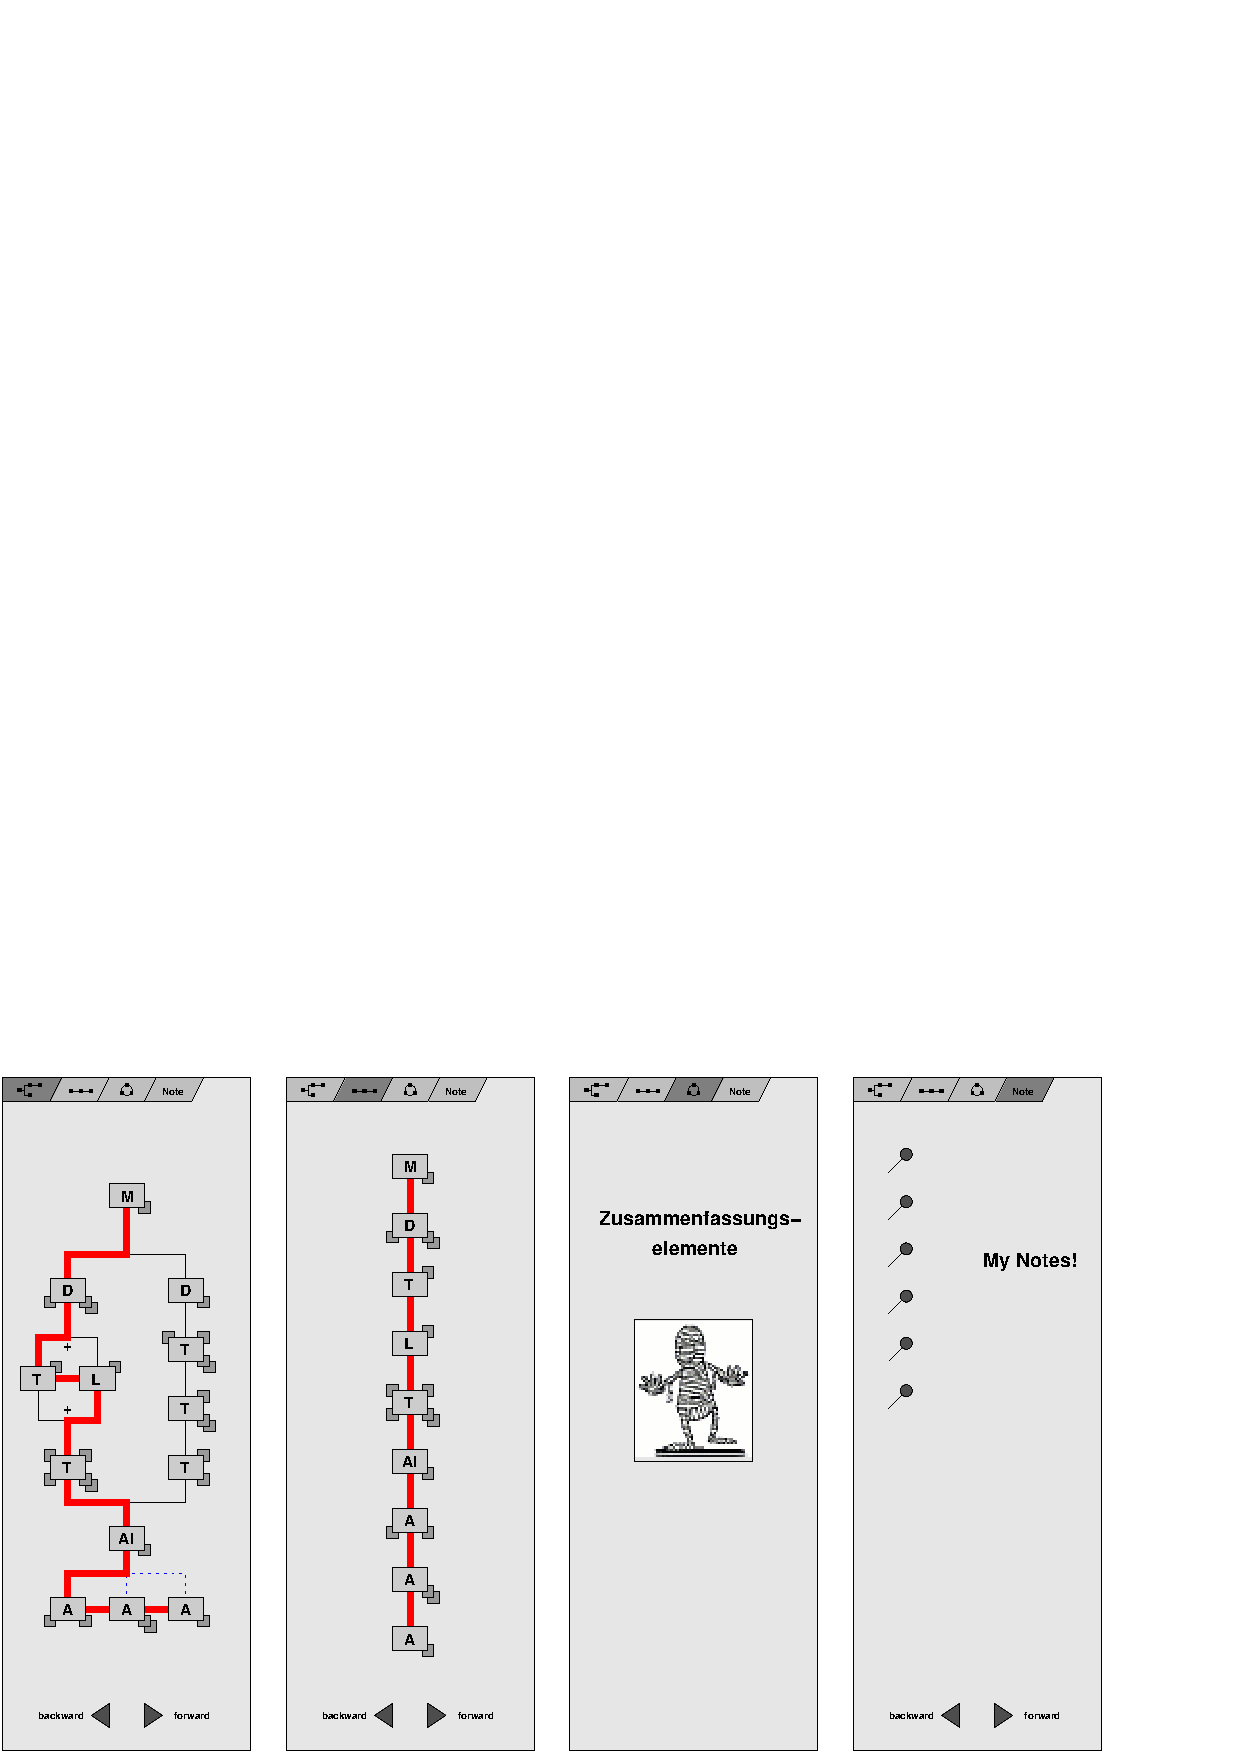
\includegraphics{Skizzen/all_cards.pdf}
\fi
\caption{Umschalten durch Karteikarten}
\end{center}
\end{figure}


%********************************************************************************

\clearpage

%********************************************************************************

\subsection{Zentrale Inhaltsfenster}


\subsubsection{Overview}


\subsubsection{Buttons}


\subsubsection{Integrierte}



\clearpage

\section{"Ubungstool}\label{lerntool}
to be specified...

\section{Lexikontool}\label{lerntool}
to be specified...

\section{Kommunikationstool}\label{lerntool}
to be specified...

\section{Weitere Tools}\label{weitere_tools}
to be specified...





%%%
\section{Overview}\label{overview}

Im Lernteil des Mumie-Projektes unterteilt sich das
\textbf{Haupt}browserfenster in folgende Bereiche:

\begin{list_sabina}
        \item \textbf{zentrale Men"uleiste} (f"ur globale Optionen)
        \item \textbf{Navigationsbereich} (f"ur die interaktive Pr"asentation des speziellen Moduls)
        \item \textbf{zentrales Inhaltsfenster} (f"ur den inhaltlichen ``Hauptinput'')
\end{list_sabina}

\begin{figure}[h]
\begin{center}
\ifx\pdfoutput\undefined
  \epsfig{file=Skizzen/gesamtszenario_01.eps, height = 5cm} 
\else
  \includegraphics{Skizzen/gesamtszenario_01.pdf}
\fi
\caption{Layout der Hauptansicht im Lerntool}
\end{center}
\end{figure}


Der Navigationsbereich wird auf zwei verschiedene Weisen realisiert:

\begin{list_sabina}
        \item \textbf{Navigationsnetz}: Die Netzdarstellung erlaubt das orientierte
          Navigieren im gew"ahlten Kurs, stellt aber zus"atzlich weitere
          Elemente und alternative Wege dar, die jederzeit mit angew"ahlt
          werden k"onnen. \\
          Die Netzstruktur dient insbesondere der Vermittlung von
          mathematischen Zusammenh"angen: die logischen Abh"angigkeiten der
          Elemente werden durch eine Strichart (``logisches Netz''), 
          der gew"ahlte Kurs durch eine zweite Strichart (``Kurspfad'')
          dargestellt. Forward/Backward-Aktionen beziehen sich stets
          auf den Kurspfad.
        \item \textbf{lineare Navigation:} Die lineare Darstellung (Modell
          etwa wie ein U-Bahn-Plan f"ur eine einzige Linie) stellt nur die
          Elemente des Modules dar, die f"ur den gew"ahlten Kurs vorgesehen
          sind. Alternative Wege und/oder weitere vorhandene Elemente sind in
          dieser Darstellung unsichtbar.\\
	  Die lineare Navigation dient insbesondere dem Ziel, dem 
	  ``Lost-in-Cyberspace''-Effekt entgegenzuwirken.
\end{list_sabina}


Ausgangspunkt f"ur die Darstellung ist zun"achst das Navigationsnetz (hier
wird auf Alternativen erst aufmerksam gemacht, deren Existenz andernfalls
nicht sichtbar ist). Zwischen den beiden Navigationsformen kann zu jeden
Zeitpunkt geswitched werden (Karteikartensytem am oberen Rand des
Navigationsbereiches).


%%%\clearpage



%***************************************************************************************

\end{document}


















